\chapter{Gráficas completas de las activaciones neuronales del grupo de agentes de tipo 1}\label{ch:anexo3}
\begin{figure}[!h]
    \centering % <-- added
\begin{subfigure}{0.33\textwidth}
  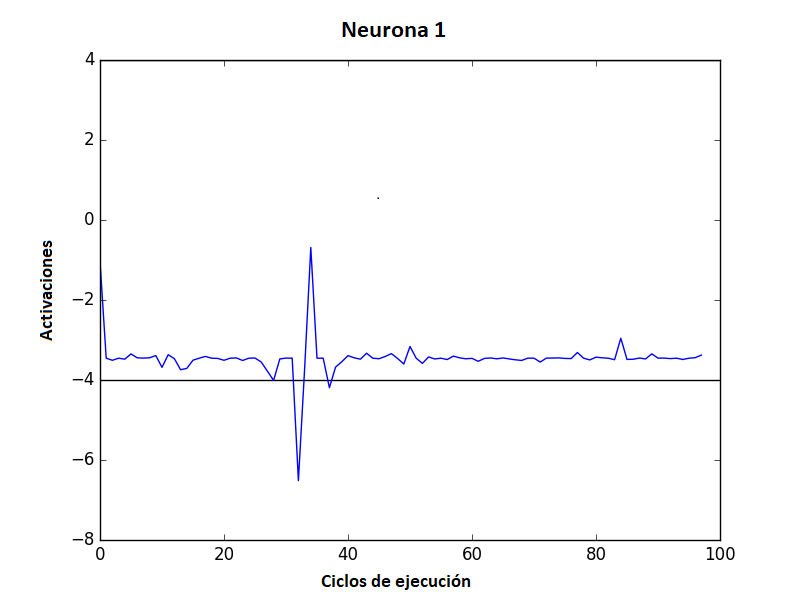
\includegraphics[width=\linewidth]{Imagenes/Agente1Activaciones/Agente0/Neurona0}
\end{subfigure}\hfil % <-- added
\begin{subfigure}{0.33\textwidth}
  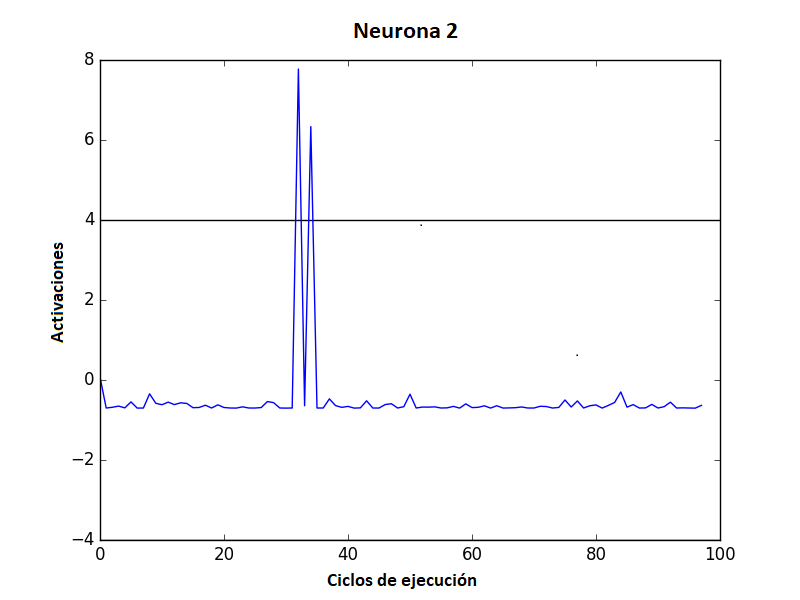
\includegraphics[width=\linewidth]{Imagenes/Agente1Activaciones/Agente0/Neurona1}
\end{subfigure}\hfil % <-- added
\begin{subfigure}{0.33\textwidth}
  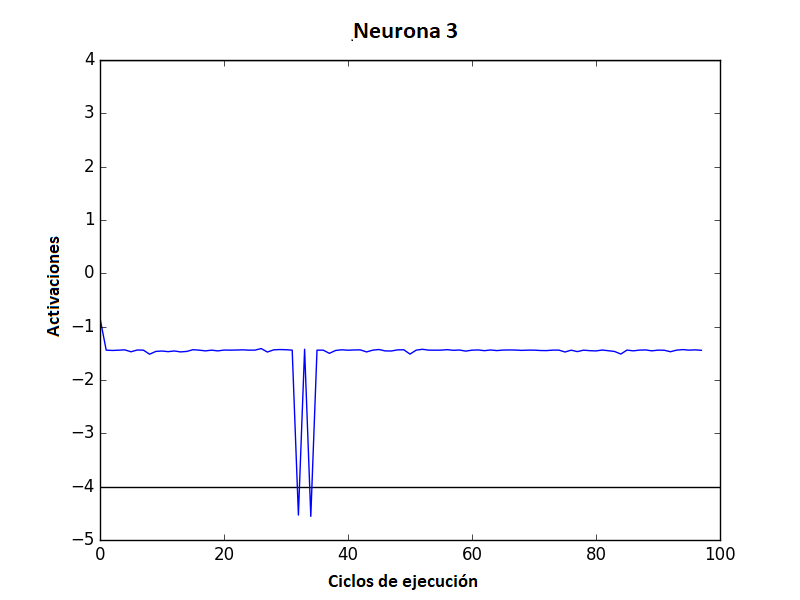
\includegraphics[width=\linewidth]{Imagenes/Agente1Activaciones/Agente0/Neurona2}
\end{subfigure}
\medskip
\begin{subfigure}{0.33\textwidth}
  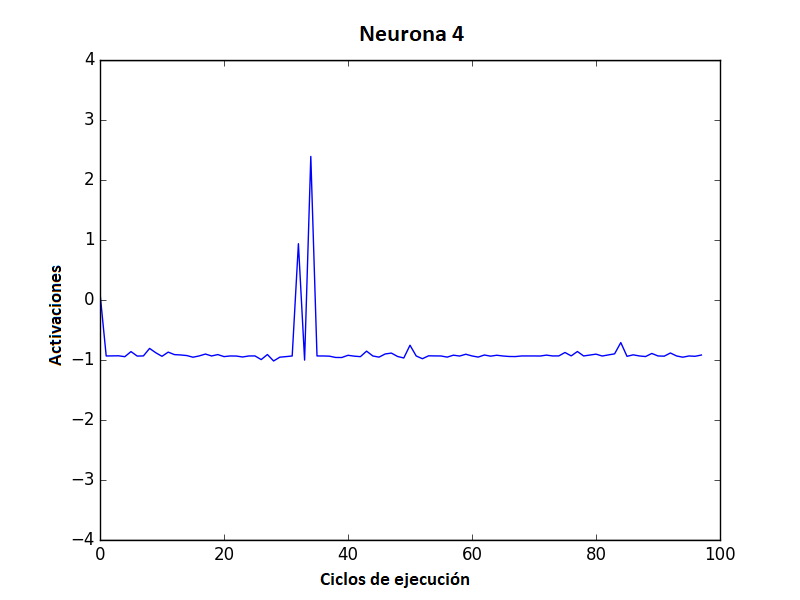
\includegraphics[width=\linewidth]{Imagenes/Agente1Activaciones/Agente0/Neurona3}
\end{subfigure}\hfil % <-- added
\begin{subfigure}{0.33\textwidth}
  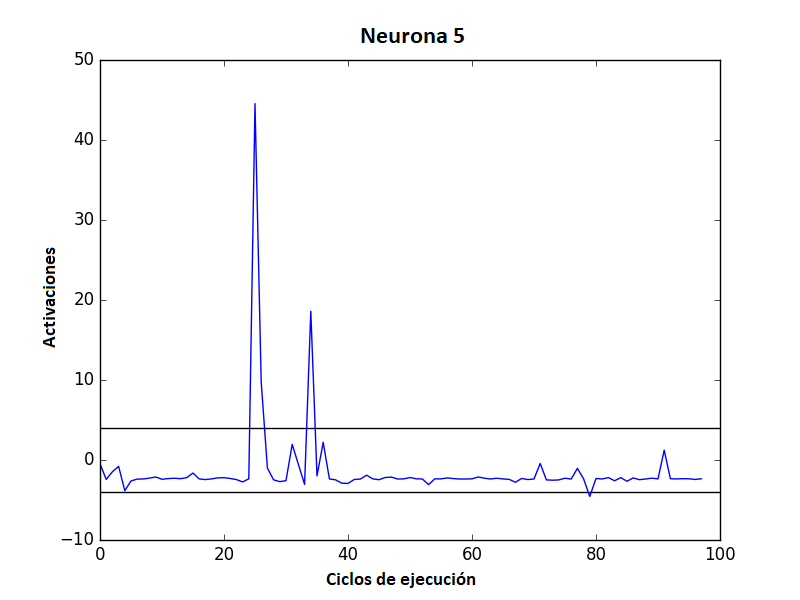
\includegraphics[width=\linewidth]{Imagenes/Agente1Activaciones/Agente0/Neurona4}
\end{subfigure}\hfil % <-- added
\begin{subfigure}{0.33\textwidth}
  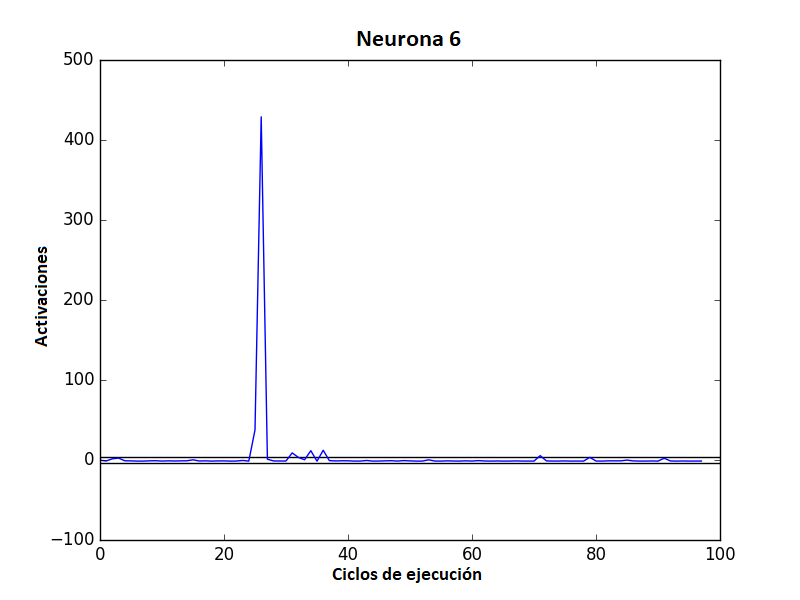
\includegraphics[width=\linewidth]{Imagenes/Agente1Activaciones/Agente0/Neurona5}
\end{subfigure}
\caption{Activaciones de las 6 neuronas del agente número 1 del tipo 1.}
\end{figure}

\begin{figure}[!h]
    \centering % <-- added
\begin{subfigure}{0.33\textwidth}
  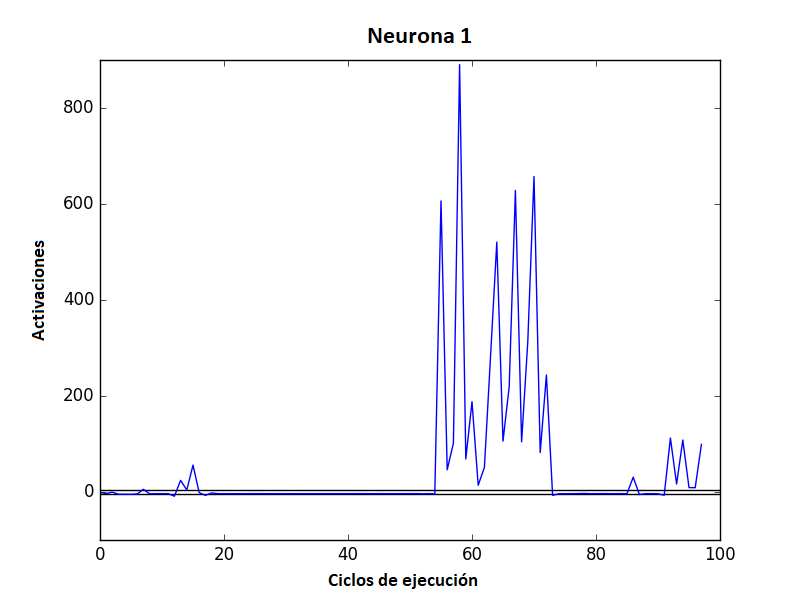
\includegraphics[width=\linewidth]{Imagenes/Agente1Activaciones/Agente1/Neurona0}
\end{subfigure}\hfil % <-- added
\begin{subfigure}{0.33\textwidth}
  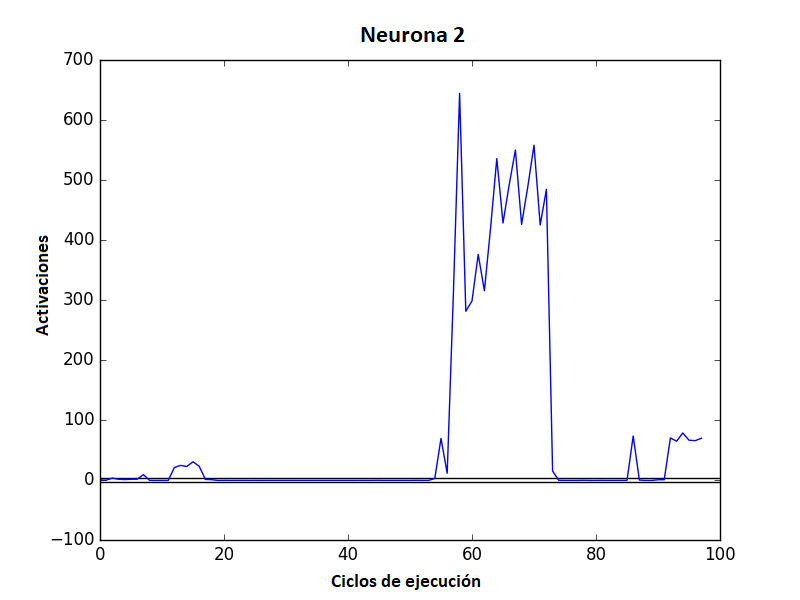
\includegraphics[width=\linewidth]{Imagenes/Agente1Activaciones/Agente1/Neurona1}
\end{subfigure}\hfil % <-- added
\begin{subfigure}{0.33\textwidth}
  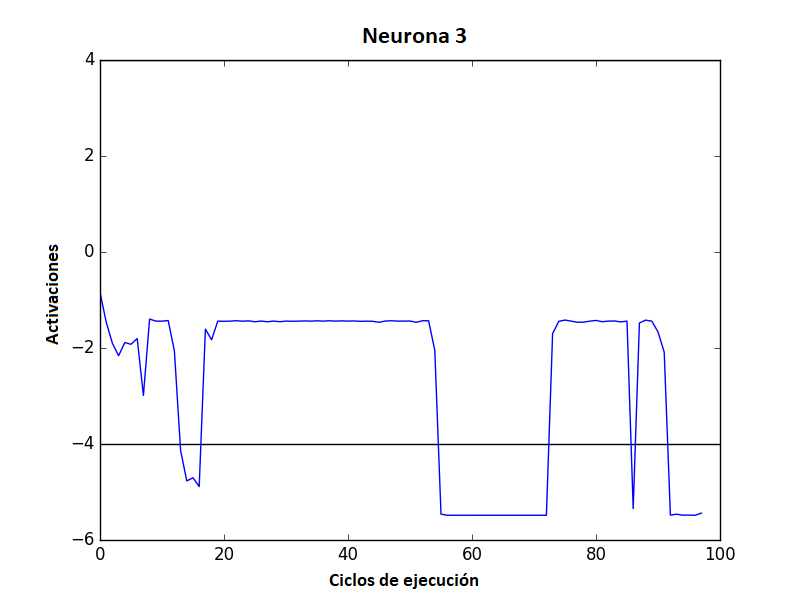
\includegraphics[width=\linewidth]{Imagenes/Agente1Activaciones/Agente1/Neurona2}
\end{subfigure}
\medskip
\begin{subfigure}{0.33\textwidth}
  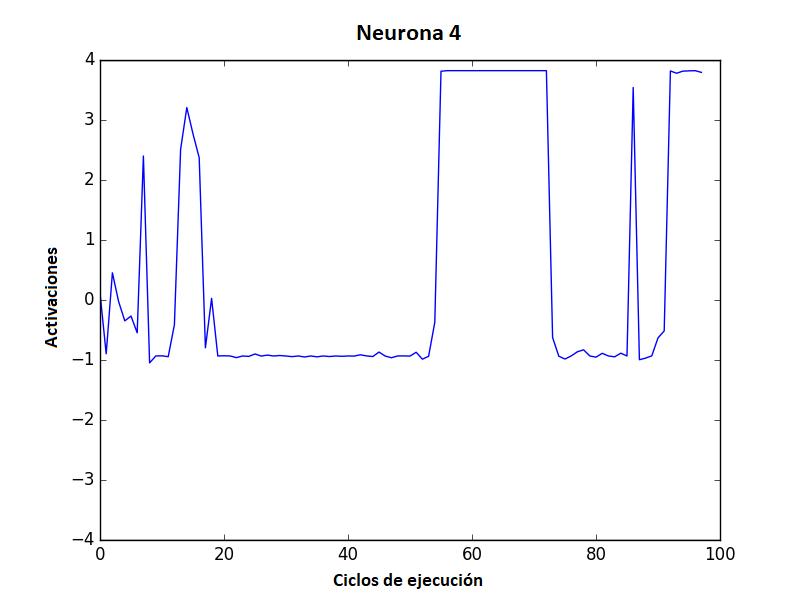
\includegraphics[width=\linewidth]{Imagenes/Agente1Activaciones/Agente1/Neurona3}
\end{subfigure}\hfil % <-- added
\begin{subfigure}{0.33\textwidth}
  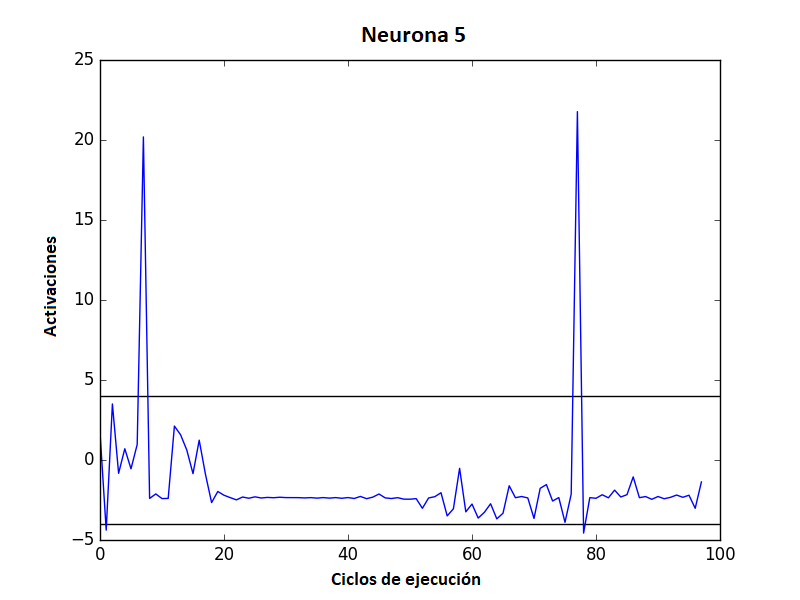
\includegraphics[width=\linewidth]{Imagenes/Agente1Activaciones/Agente1/Neurona4}
\end{subfigure}\hfil % <-- added
\begin{subfigure}{0.33\textwidth}
  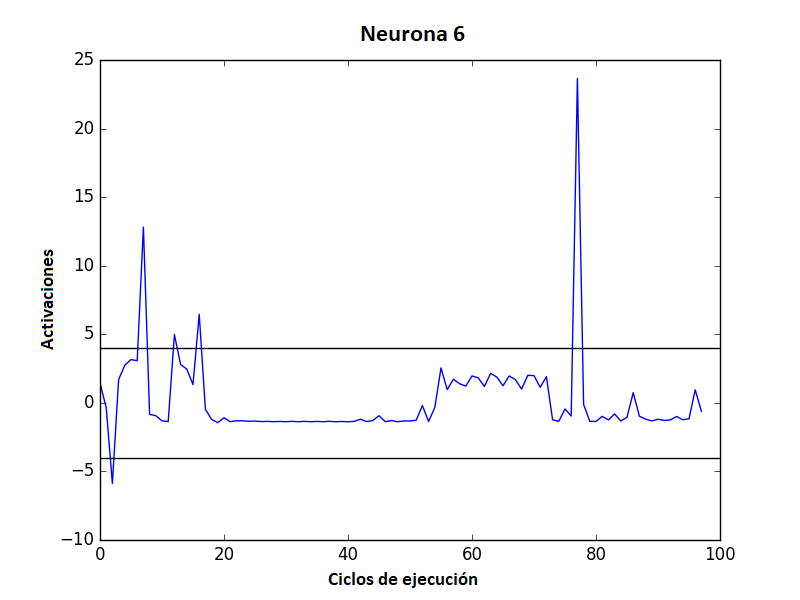
\includegraphics[width=\linewidth]{Imagenes/Agente1Activaciones/Agente1/Neurona5}
\end{subfigure}
\caption{Activaciones de las 6 neuronas del agente número 2 del tipo 1.}
\end{figure}

\begin{figure}[!h]
    \centering % <-- added
\begin{subfigure}{0.33\textwidth}
  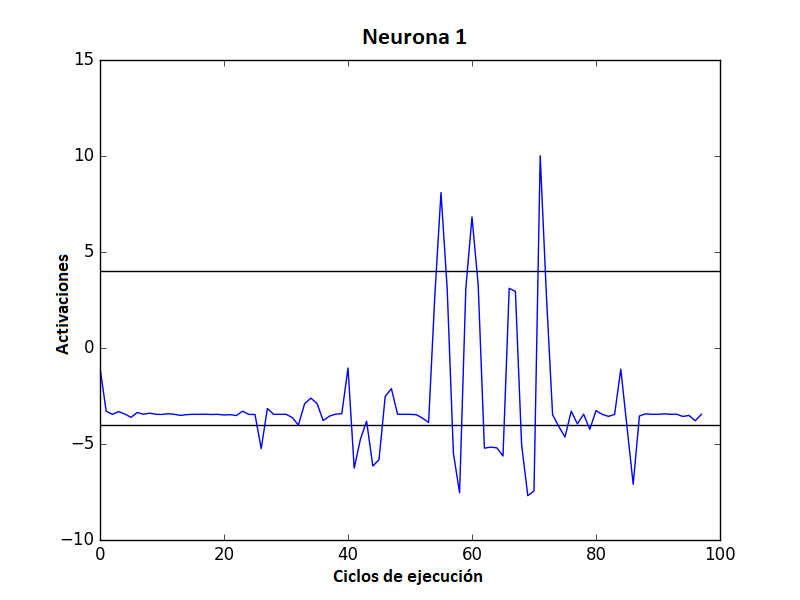
\includegraphics[width=\linewidth]{Imagenes/Agente1Activaciones/Agente2/Neurona0}
\end{subfigure}\hfil % <-- added
\begin{subfigure}{0.33\textwidth}
  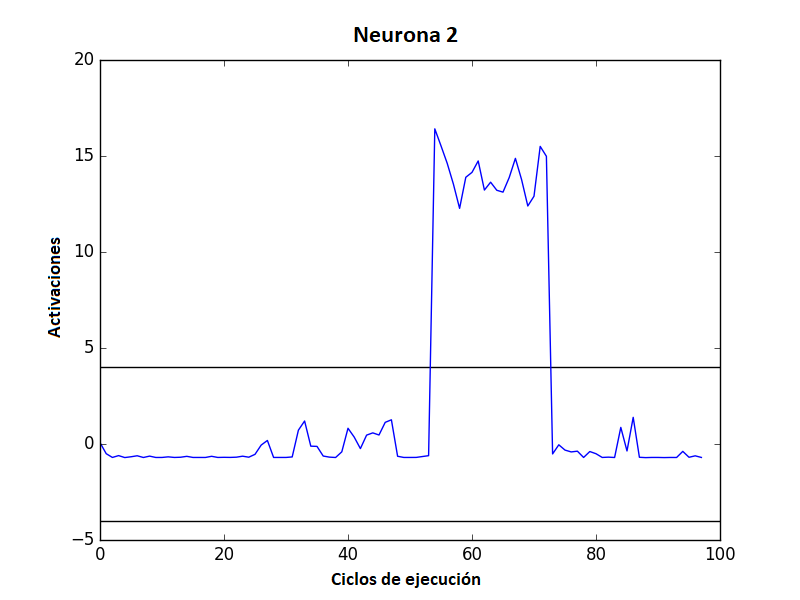
\includegraphics[width=\linewidth]{Imagenes/Agente1Activaciones/Agente2/Neurona1}
\end{subfigure}\hfil % <-- added
\begin{subfigure}{0.33\textwidth}
  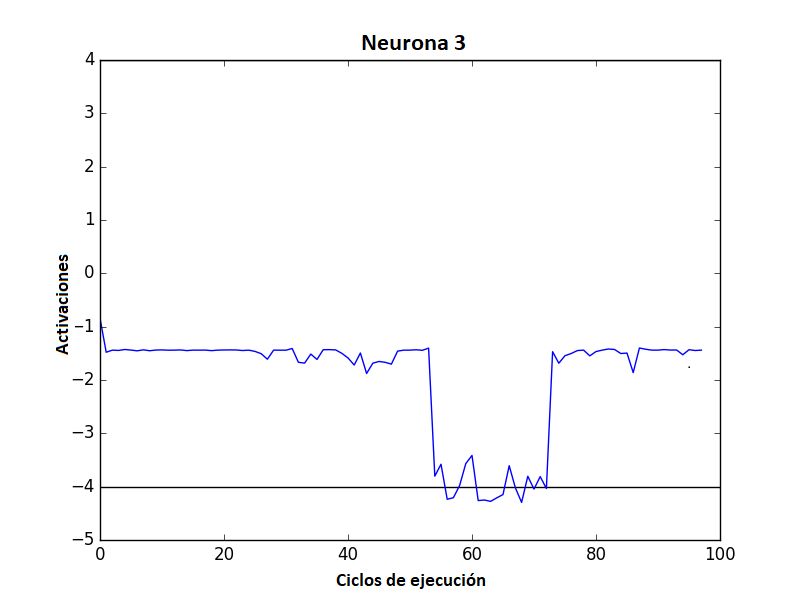
\includegraphics[width=\linewidth]{Imagenes/Agente1Activaciones/Agente2/Neurona2}
\end{subfigure}
\medskip
\begin{subfigure}{0.33\textwidth}
  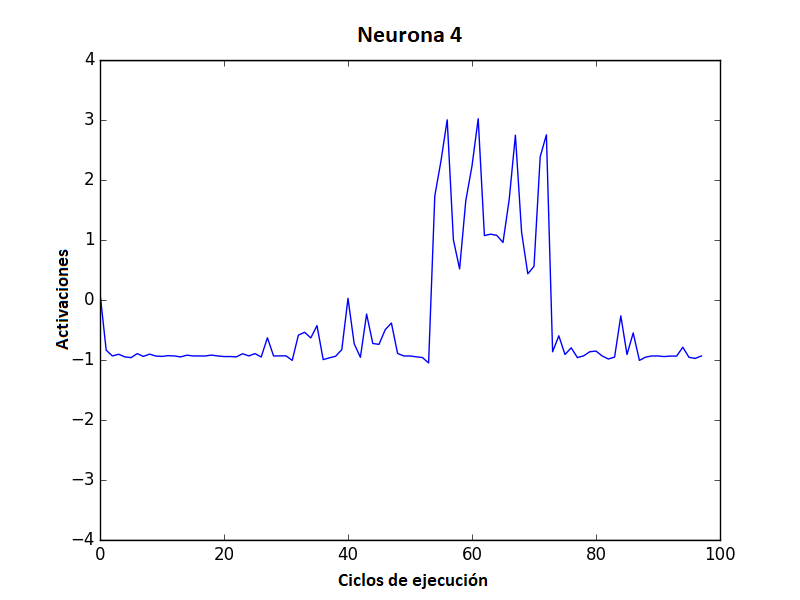
\includegraphics[width=\linewidth]{Imagenes/Agente1Activaciones/Agente2/Neurona3}
\end{subfigure}\hfil % <-- added
\begin{subfigure}{0.33\textwidth}
  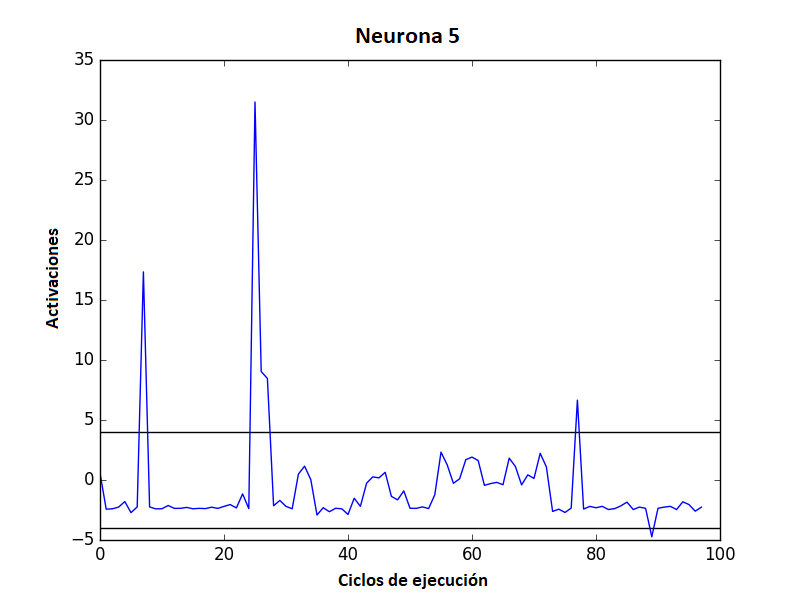
\includegraphics[width=\linewidth]{Imagenes/Agente1Activaciones/Agente2/Neurona4}
\end{subfigure}\hfil % <-- added
\begin{subfigure}{0.33\textwidth}
  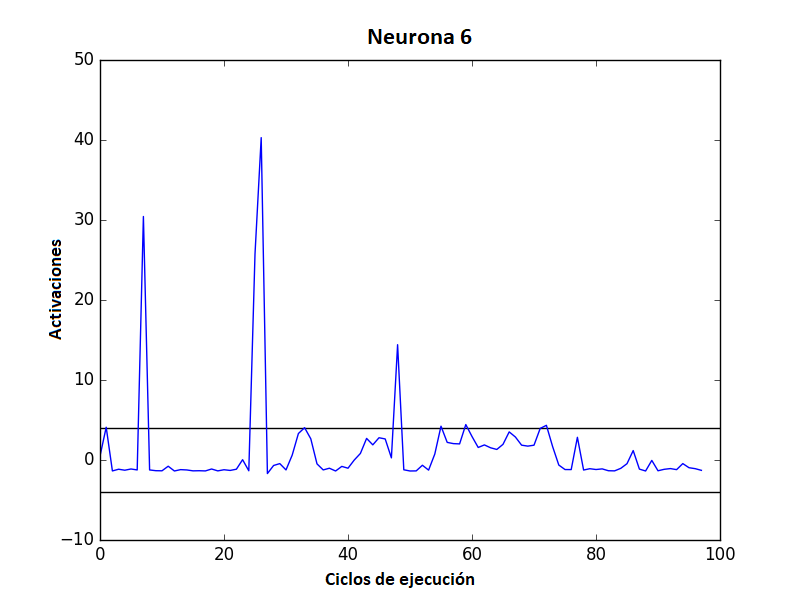
\includegraphics[width=\linewidth]{Imagenes/Agente1Activaciones/Agente2/Neurona5}
\end{subfigure}
\caption{Activaciones de las 6 neuronas del agente número 3 del tipo 1.}
\end{figure}

\begin{figure}[!h]
    \centering % <-- added
\begin{subfigure}{0.33\textwidth}
  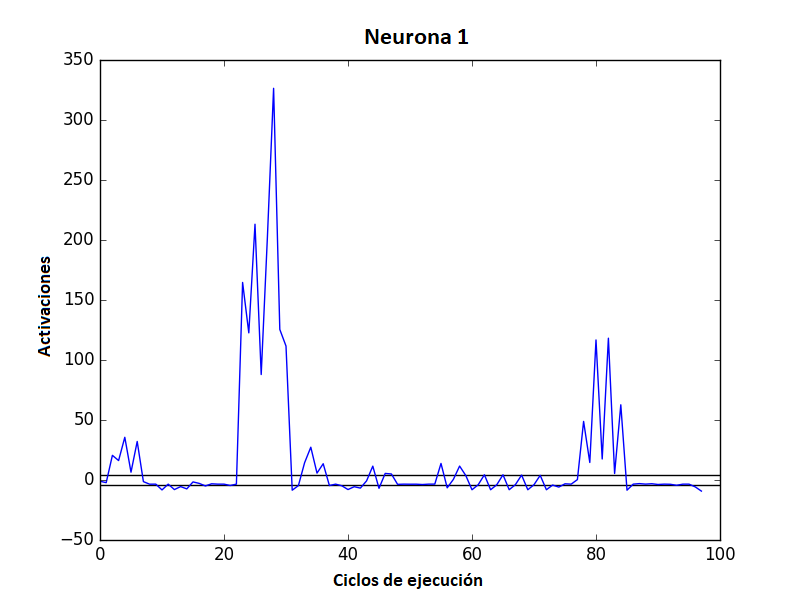
\includegraphics[width=\linewidth]{Imagenes/Agente1Activaciones/Agente3/Neurona0}
\end{subfigure}\hfil % <-- added
\begin{subfigure}{0.33\textwidth}
  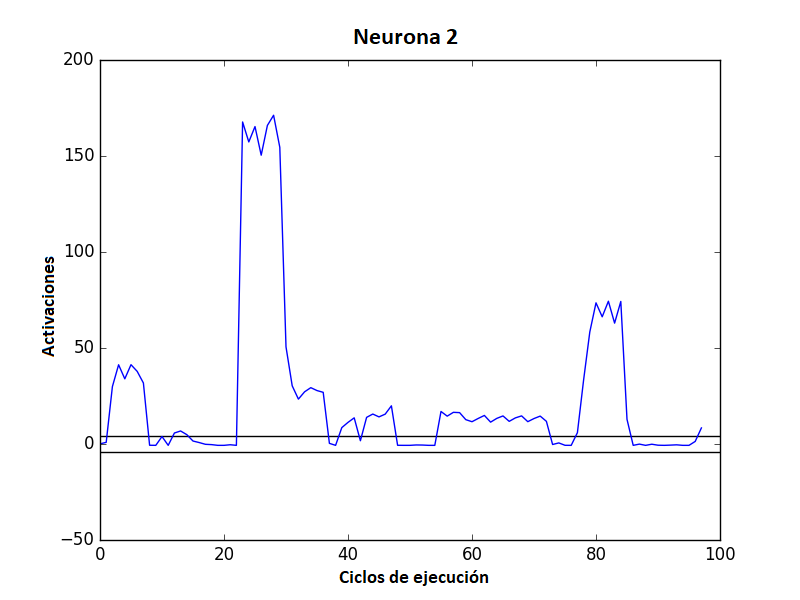
\includegraphics[width=\linewidth]{Imagenes/Agente1Activaciones/Agente3/Neurona1}
\end{subfigure}\hfil % <-- added
\begin{subfigure}{0.33\textwidth}
  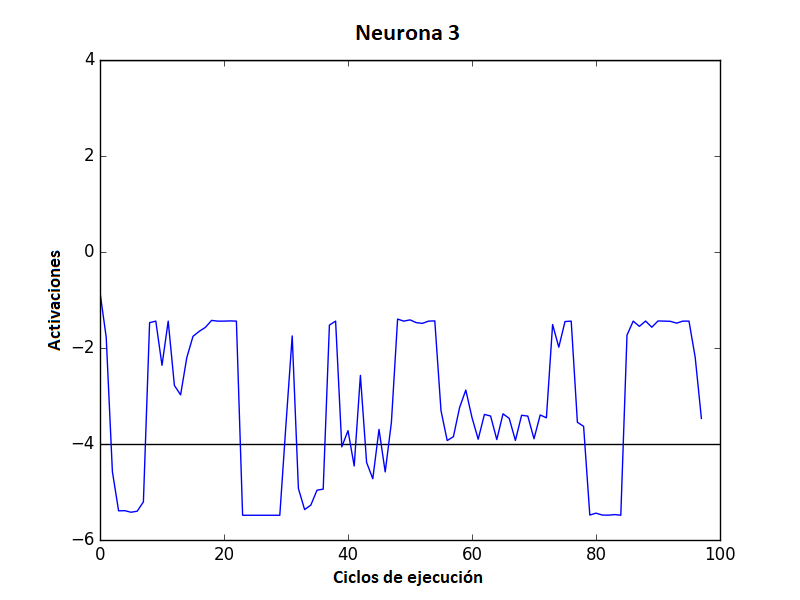
\includegraphics[width=\linewidth]{Imagenes/Agente1Activaciones/Agente3/Neurona2}
\end{subfigure}
\medskip
\begin{subfigure}{0.33\textwidth}
  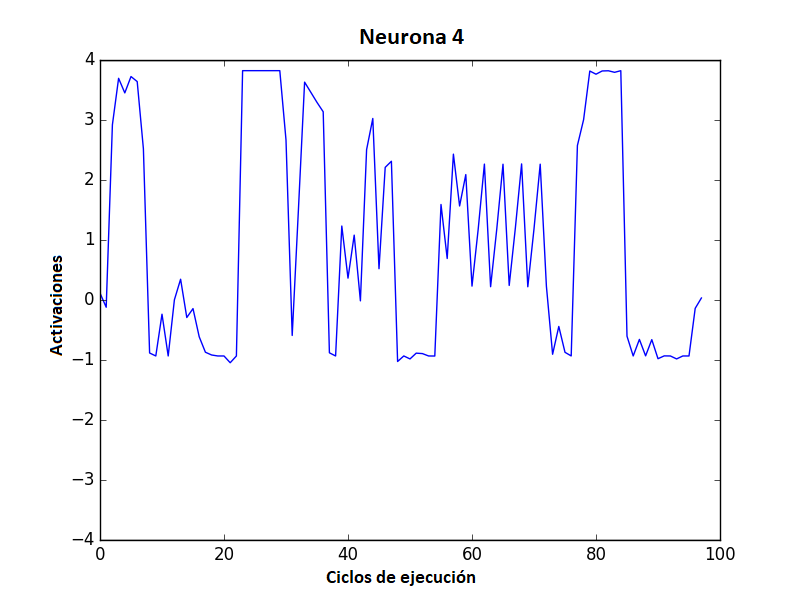
\includegraphics[width=\linewidth]{Imagenes/Agente1Activaciones/Agente3/Neurona3}
\end{subfigure}\hfil % <-- added
\begin{subfigure}{0.33\textwidth}
  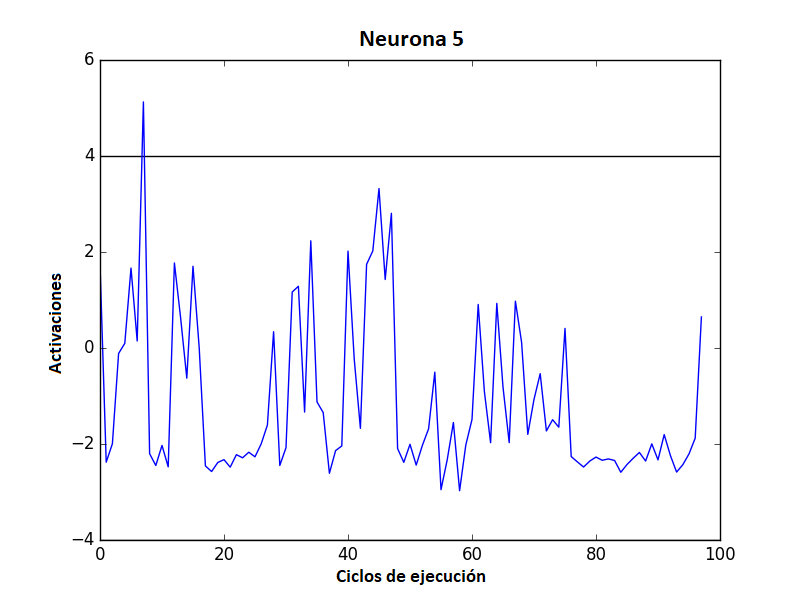
\includegraphics[width=\linewidth]{Imagenes/Agente1Activaciones/Agente3/Neurona4}
\end{subfigure}\hfil % <-- added
\begin{subfigure}{0.33\textwidth}
  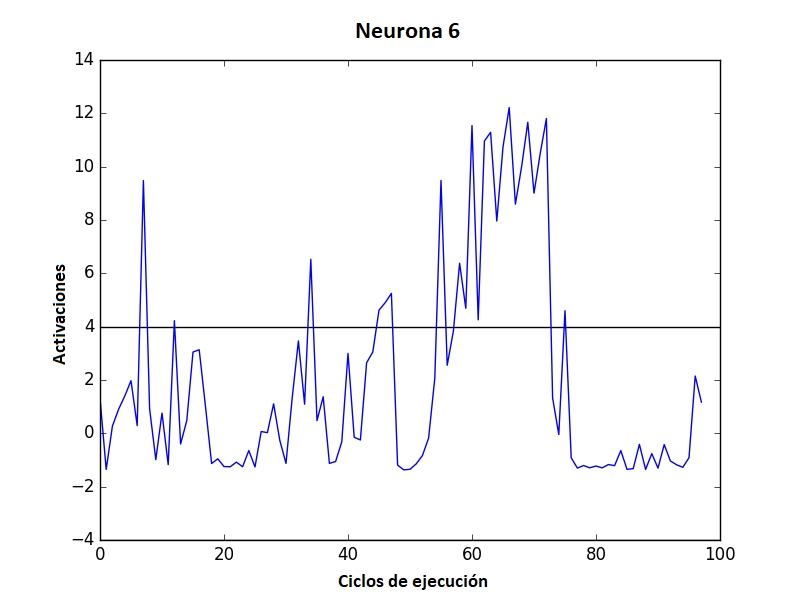
\includegraphics[width=\linewidth]{Imagenes/Agente1Activaciones/Agente3/Neurona5}
\end{subfigure}
\caption{Activaciones de las 6 neuronas del agente número 4 del tipo 1.}
\end{figure}

\begin{figure}[!h]
    \centering % <-- added
\begin{subfigure}{0.33\textwidth}
  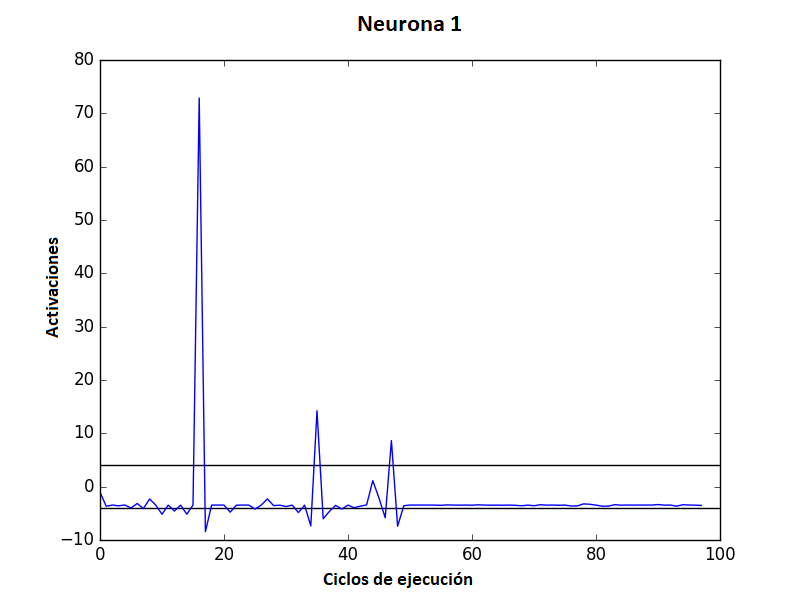
\includegraphics[width=\linewidth]{Imagenes/Agente1Activaciones/Agente4/Neurona0}
\end{subfigure}\hfil % <-- added
\begin{subfigure}{0.33\textwidth}
  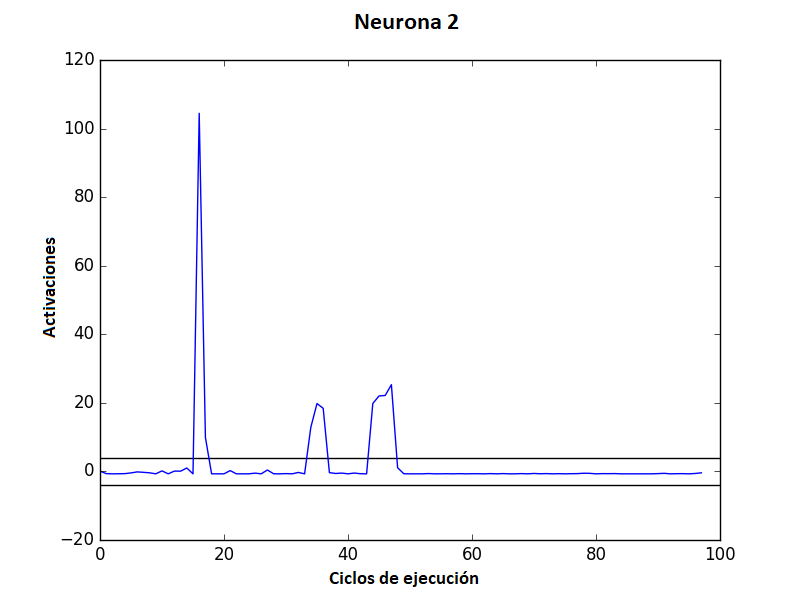
\includegraphics[width=\linewidth]{Imagenes/Agente1Activaciones/Agente4/Neurona1}
\end{subfigure}\hfil % <-- added
\begin{subfigure}{0.33\textwidth}
  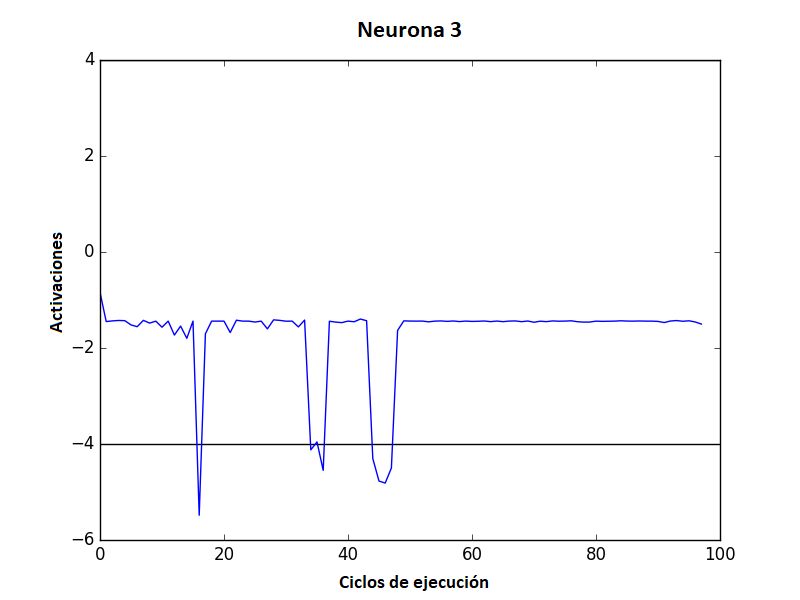
\includegraphics[width=\linewidth]{Imagenes/Agente1Activaciones/Agente4/Neurona2}
\end{subfigure}
\medskip
\begin{subfigure}{0.33\textwidth}
  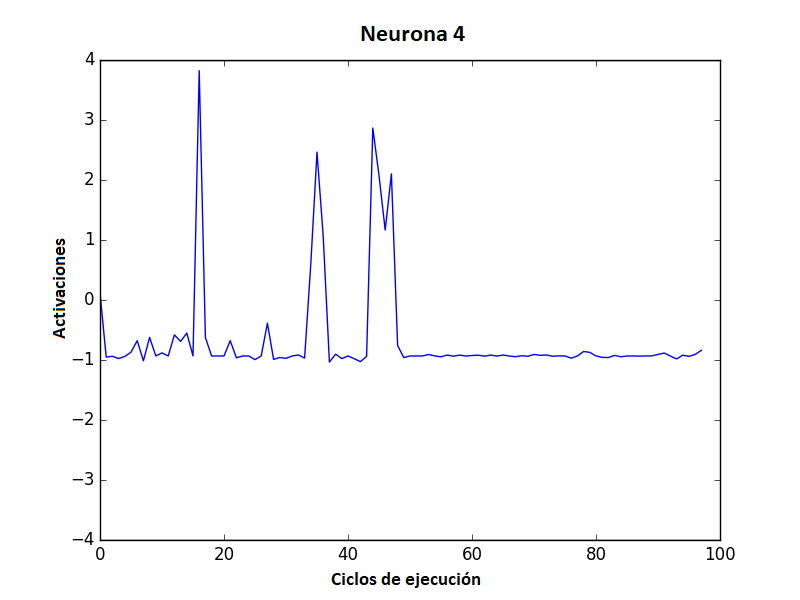
\includegraphics[width=\linewidth]{Imagenes/Agente1Activaciones/Agente4/Neurona3}
\end{subfigure}\hfil % <-- added
\begin{subfigure}{0.33\textwidth}
  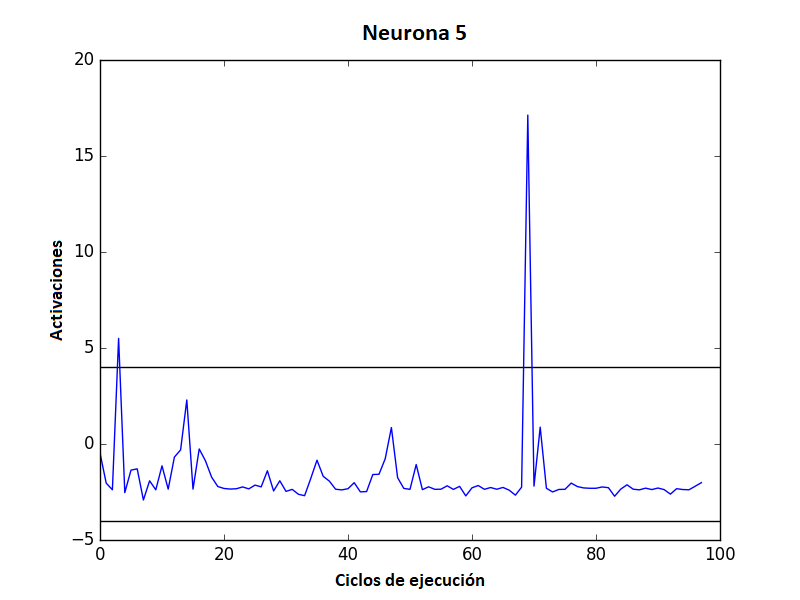
\includegraphics[width=\linewidth]{Imagenes/Agente1Activaciones/Agente4/Neurona4}
\end{subfigure}\hfil % <-- added
\begin{subfigure}{0.33\textwidth}
  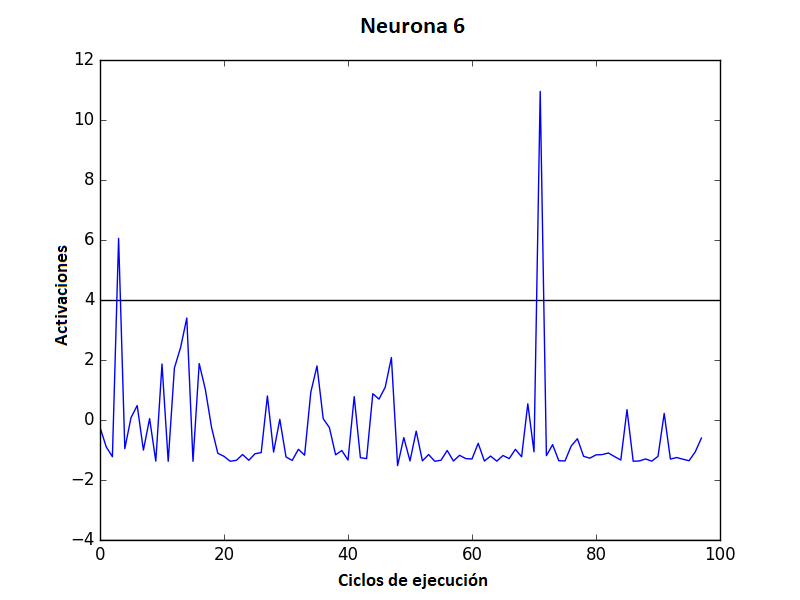
\includegraphics[width=\linewidth]{Imagenes/Agente1Activaciones/Agente4/Neurona5}
\end{subfigure}
\caption{Activaciones de las 6 neuronas del agente número 5 del tipo 1.}
\end{figure}
